\section{Experiments}

We connect our theory to pratical problems of interest.
First, we validate the single-task based metric on text and image classification tasks.
We show that for both datasets, single-task learning results can help predict positive or negative transfer in multi-task learning.
Second, \todo{}.
Third, we measure the data efficiency ratio of multi-task learning on six sentiment analysis tasks.
Finally, we validate the three components of our theory in Section \ref{sec_insight} on text classification tasks.

\begin{table}
\begin{minipage}[t]{.58\textwidth}
	\centering
  \begin{tabular}{c c c c c}
	\toprule
		\multirow{2}{*}{{\bf Threshold}}  & \multicolumn{2}{c}{{\bf Text
		classification}} & \multicolumn{2}{c}{{\bf ChestX-ray14}} \\
		& Precision &  Recall & Precision &  Recall \\
		\cmidrule(lr){1-1} \cmidrule(lr){2-3} \cmidrule(lr){4-5}
		0.0 & 0.596 & 1.000 & 0.593 & 1.000 \\
		0.1 & 0.756 & 0.388 & 0.738 & 0.462 \\
		0.2 & 0.919 & 0.065 & 0.875 & 0.044 \\
		% 0.3 & 1.000 & 0.004 &     - &     - \\
	\bottomrule
	\end{tabular}
	\vspace{0.1in}
	\captionof{table}{Single-task learning results can help predict postive or negative transfer in multi-task learning.}
	\label{tab:mtl_better_than_stl}
\end{minipage}
\quad
% \vspace{}
\begin{minipage}[t]{.40\textwidth}
	\centering
	\begin{tabular}{c c c}
		\toprule
		\multirow{2}{*}{{\bf Models}} & \multicolumn{2}{c}{\begin{minipage}{1.1in}\begin{center}
		MR, SST, SUBJ, CR, MPQA, TREC\end{center}\end{minipage}} \\
		\cmidrule(lr){2-3}
		& {\bf Standard} & {\bf Alignment} \\
		\midrule
		{\bf MLP}  & > 100\% & 39\% \\
		{\bf LSTM} & 36\% & 36\% \\
		\bottomrule
		\end{tabular}
	\vspace{0.1in}
	\captionof{table}{Measuring the data efficiency ratio of muli-task learning.}
	\label{tab:taskonomy}
\end{minipage}
\end{table}

\subsection{Experimental Setup}

{\bf Datasets and models.} We describe the datasets and models we use in the experiments.

{\it Sentiment Analysis:} This dataset includes six tasks: movie review sentiment (MR), sentence subjectivity (SUBJ), customer reviews polarity (CR), question type (TREC), opinion polarity (MPQA), and the Stanford sentiment treebank (SST) tasks.

{For each task, the goal is to categorize sentiment opinions expressed in the text.
We use an embedding layer (with GloVe embeddings\footnote{http://nlp.stanford.edu/data/wordvecs/glove.6B.zip}) followed by an LSTM layer proposed by~\cite{lei2018simple}.
}
%multi-layer perceptron (MLP), LSTM, CNN on all tasks
%We use this task to verify our theoretical results on model capacity and task covariance in real world.

{\it ChestX-ray14:} This dataset contains 112,120 frontal-view X-ray images and each image has up to 14 diseases.
This is a 14-task multi-label image classification problem.
%We treat each label as one task a binary classification problem and formulate it as a 14-task multi-task learning problem.
%This dataset is curated where the labels
%We use the CheXNet model from~\cite{chexnet}, which is a 121-layer convolutional neural network on all tasks.

For all models, we share the main module across all tasks and assign a separate regression or classification layer on top of the shared module for each tasks.



\subsection{Experimental Results}

\textbf{Understanding MTL results via STL results.}
We show that STL results can be used to help understand MTL results
We validate the single-task based metric proposed in Section \ref{sec_similarity} for predicting positive or negative transfer in MTL.
Table \ref{tab:mtl_better_than_stl} shows the result on both the sentiment analysis and the ChestX-ray14 datasets.
We find that using a threshold of $\tau = 0.1$, the STL results correctly predict positive or negative transfer with $75.6\%$ accuracy and $38.8\%$ recall among 150 task pairs.
We observe similar results for 91 task pairs from the ChestX-ray14 dataset.
The results show that STL performances are indicative of MTL performances.

\textbf{Improving training efficiency via an incremental schedule.}
\todo{}

\textbf{MTL improves labeled data efficiency.}
We measure the data efficiency ratio on the sentiment analysis tasks.
In Table \ref{tab:taskonomy}, we find that by performing multi-task learning, only $39\%$ of the labeled data is needed to achieve comparable performance to single-task learning over all six tasks on LSTM.
We further observe that adding the alignment module helps reduce the data efficiency ratio on MLP.
%If TREC is not included, we see that only $25\%$ of the labeled data is needed.


\subsection{Ablation Studies}


\textbf{Task similarity.} We validate that MTL performs better when the source task is more similar to the target task.
We show the result on the sentiment analysis tasks.
For a target task, we manually select a similar task and a dissimilar task based on prior knowledge.
Figure \ref{fig_ab_sim} confirms the result.


\textbf{Data size.}
Recall that Section \ref{sec_data_size} shows that increasing the data size of the source task does not always improve the performance of MTL for the target task.
In Figure \ref{fig_ab_data}, we show that for source task MR and target task SST, there is a transition from positive to negative transfer as we increase the data size of the source task.

\textbf{Covariate shift.}
%Our result provides a fine-grained insight on the covariance alignment algorithm proposed in \cite{WZR20}.
%Recall that the covariance alignment procedure in \cite{WZR20} adds an additional module between the word embedding representation and the shared module.
When the source task data size is particularly large compared to the target task, we show that applying the covariance alignment algorithm results in more significant gains.
In Figure \ref{fig_ab_cov}, we observe that the benefit from aligning task covariances becomes more significant for LSTM and MLP as we increase the number of datapoints of the source task.


\begin{figure}[!t]
	\centering
	\begin{subfigure}[b]{0.33\textwidth}
		\centering
		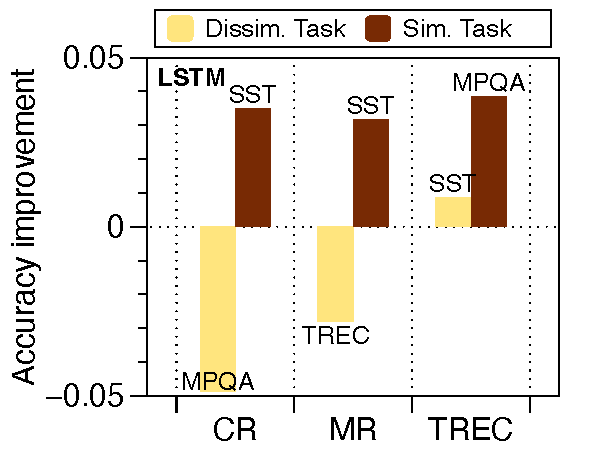
\includegraphics[width=0.975\textwidth]{figures/task_sim_norm_lstm.pdf}
		\caption{Task similarity}
		\label{fig_ab_sim}
	\end{subfigure}%
	\begin{subfigure}[b]{0.33\textwidth}
		\centering
		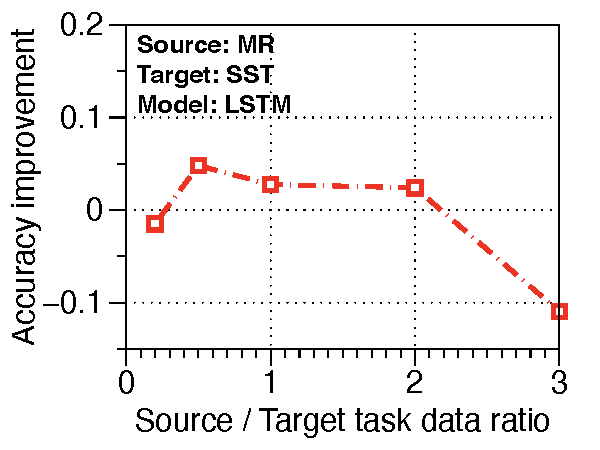
\includegraphics[width=0.975\textwidth]{figures/ratio_norm_sst_trec_lstm.pdf}
		\caption{Data size}
		\label{fig_ab_data}
	\end{subfigure}
	\begin{subfigure}[b]{0.33\textwidth}
		\centering
		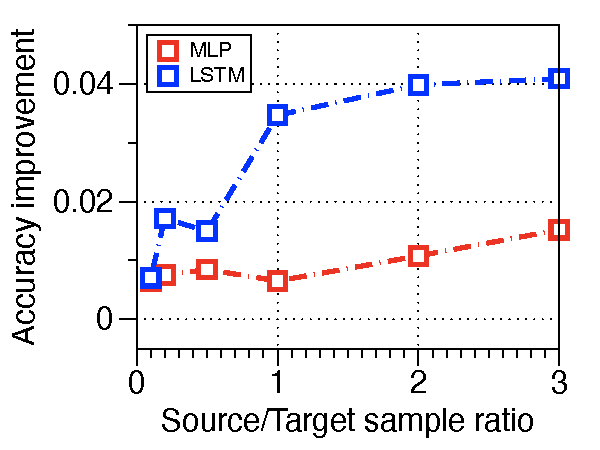
\includegraphics[width=0.975\textwidth]{figures/ratio_alignment_norm_diff_all.pdf}
		\caption{Covariate shift}
		\label{fig_ab_cov}
	\end{subfigure}
	\caption{Validating the three takeaways of Section \ref{sec_insight} on sentiment analysis tasks. (a) Adding a semantically similar source task in MTL performs better than adding a dissimilar task.
	(b) As source/target data ratio increases, we observe a transition from positive to negative transfer.
	(c) As source/target data ratio increases, the performance gains from the covariance alignment procedure \cite{WZR20} increase for LSTM and MLP.
	The $y$-axis measures the performance of MTL minus STL.}
	\label{fig_ablation}
\end{figure}

